\section{Firewall \& IDS/IPS}

\pgra{Definition:} A firewall is a hardware or software device which is configured to permit, deny or proxy data through a computer network which has different levels of trust. The configuration is called a policy.

\pgra{Filtering:} ingress (incoming traffic), egress (outgoing traffic). \textit{Default policy:} accept or reject. \textit{Deny access:} drop: silently drop packet, reject: drop packet and inform sender with ICMP

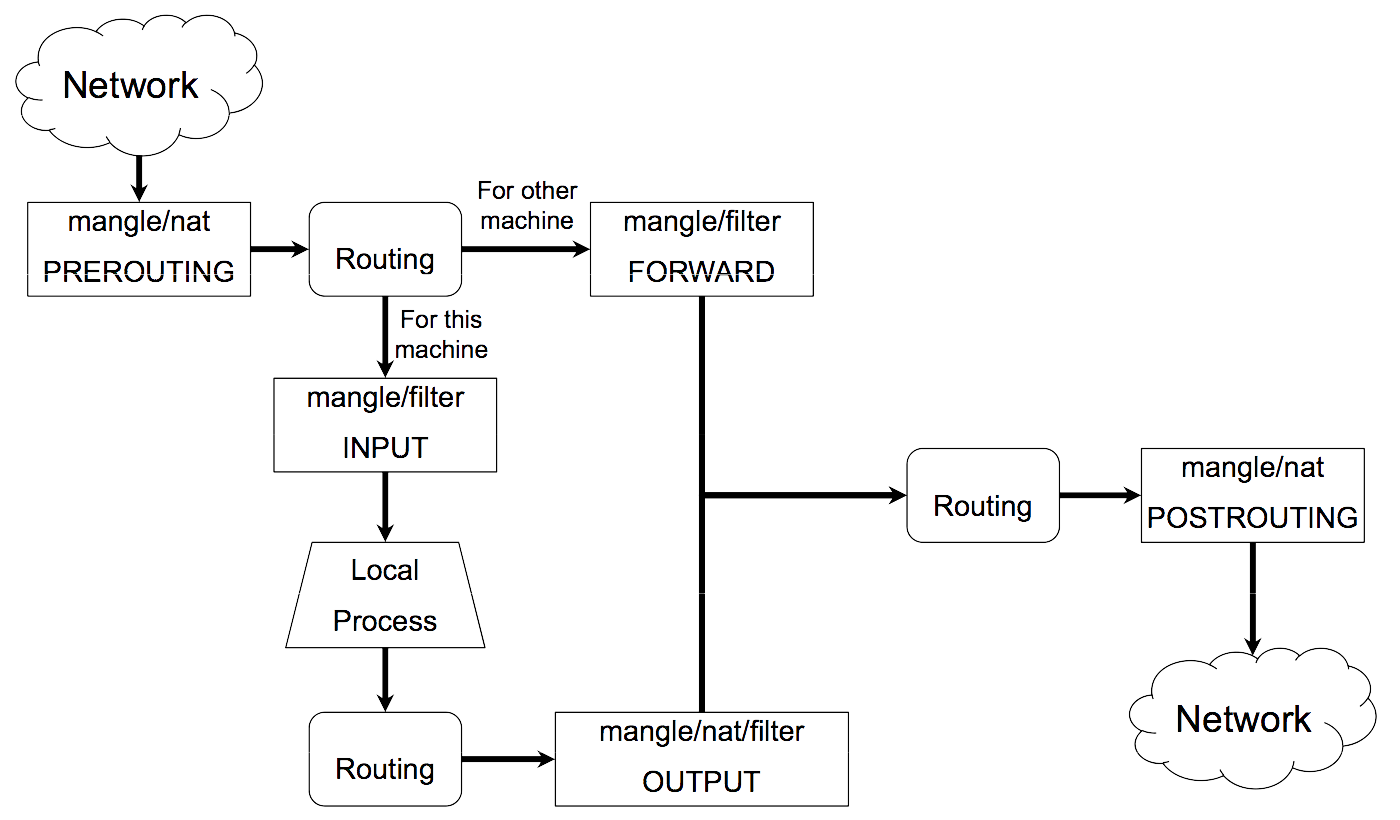
\includegraphics[width=9cm]{images/netfilter}

\pgra{Firewall configuration} Netfilter (Linux packet filter), use {\tt iptables} to configure (can do deep packet inspection, examine state, NAT). Firewall contains chains, linked to tables, that contain rules. \\
Preconfigured tables: filter (drop or accept), NAT (change src. or dst. address), mangle (change packet in more generalised ways), raw (specialised processing).\\
Rule targets: accept, drop, queue, return, masquerade (only NAT). Examples: \\
{\tt iptables -A -i eth0 -m state --state ESTABLISHED,}\\
{\tt RELATED -j ACCEPT ... -p tcp -s 0/0 -d 0/0}\\
{\tt --destination -port 80 --syn -j ACCEPT}

\pgra{Firewall commands:} and description

\begin{tabular}{p{0.35\linewidth}p{0.6\linewidth}}
Command & Description \\
\hline
\hline
ACCEPT & Accept packet \\
DROP & Discard packet \\
QUEUE & Hand packet off to userspace process \\
RETURN & Stop processing in this chain, return to previous \\
MASQUERADE & only in nat table: rewrite src. or dest. address with that of outgoing/incoming address \\
\end{tabular}

\pgra{Organizational Challenges:} Large rulesets, big organizations, conflicting goal: networking (provides connectivity) vs. security staff (protect and disrupt connectivity).

\lbtab{0.4}{0.25}{0.25}{
Type & Advantage & Disadvantage \\
\hline
\hline
\textbf{Stateless FW:} packet examination at network layer, decision based on packet header & Application independent. Good performance and scalability & No state or appl. context \\
\hline
\textbf{Stateful FW:} track-keeping of the state of network connections. Decisions are based on session state. & Easier to specify rules & State explosion. UDP is stateless! \\
\hline
\textbf{Application layer FW:} take appl. state into security decision. & Appl. awareness & Needs to support many appl. protocols. Performance, scalability \\
}

\pgra{Web Application Firewall:} Protect web based applications from malicious requests (SaaS).
\\ Request filtering:
\bitem{
\item Request patterns (SQL injection, XSS, etc.)
\item Static or dynamic blacklisting/whitelisting
\item False positive problem
}

\pgra{Firewall attack/bypass techniques:}
\bitem{
\item IP source address spoofing (doesn't work against TCP - handshake)
\item Artificial Fragmentation (port no. only in first fragment or overwritten - requires full reassembly)
\item Explot Vulnerabilities (in firewall SW/OS or target appl.)
\item DoS (State explosion - FW fallback policy?)
\item Tunneling/Covert Channel (use ICMP ping packets/DNS requests)
}

\pgra{Firewall detection by port scanning:}
\bitem{
\item Port scanning: identify potential firewall IP via traceroute, port scan targets, analyze response (check source IP address of responses of blocked/open ports, analyze differences in responses)
\item Firewall detection avoidance: Firewall improves obscurity by spoofing src of RST/ACK packet to be that of target host
}

\pgra{Firewall detection by exceeding TTL:} set packet TTL to expire one hop past firewall, if packet passes the firewall, a TTL expired should be received, if packet is blocked either ICMP is received or packet is dropped without comment.

\pgra{Firewall detection evasion:} Firewall checks for low TTL, spoofs or creates response )trying to keep existence of firewall a secret is not a security technique).

Implementation often as a reverse proxy client outside the internal network.

\pgra{NAT:} Enable multiple hosts on a private network to access the internet using a single public IP. Rewrite src./dst. address. 
\bitem{
\item[+] Prevents malicious activity initiated by outside host
\item[+] Saves address space 
\item[-] No true end-to-end connectivity
\item[-] Some protocols can be disrupted (IPSec, SIP, FTP...) 
\item[-] No protection against insider attacks
\item[-] Not suitable for service to outside
}

Modes: 1.Basic NAT (1 to 1), 2. Network Address and Port Translation (many to 1)

\pgra{NAT concept:} IP-to-port-mapping, session endpoint: (IP:Port), session defined by its 2 endpoints, direction is the flow direction of packet that initiates session (initial SYN packet for TCP, first user datagram for UDP).

\pgra{NAT example} IPtables has a NAT table in OUTPUT and POSTROUTING chains, which supports MASQUERADE jump (replace sender address with router address).

\pgra{NAT UDP hole punching:} assumes that client A and B already have active connection with a rendezvous server S, A asks S for help to establish connection with B, S replies with B's endpoints, S sends B connection request with A's endpoints. A and B start sending UDP packets: 1st packet from A punches hole in A's NAT and is blocked by B, 1st packet from B punches hole in B's NAT and passes A's NAT, 2nd packet from A passes B's NAT.

\pgra{STUN - Session Traversal Utilities for NAT:} Solves problem of discovering external address, client needs address of STUN server, client sends binding request to STUN server by UDP, receives his external address in the response (if NAT does deep packet inspection and rewrites anything that looks like my IP $\to$ XOR-ing with fixed mask), will not work with symmetric NATs that remember the remote end of UDP packet.

\pgra{IDS/IPS:} Protection inside the security perimeter.\\
\emph{Intrusion detection:} try to detect intrusions on the network, traffic compared to database of attack signatures, various methods exist.\\
\emph{Intrusion prevention:} selectively blocks traffic after detection.
\emph{IDS/IPS output:} Alerts, many false positives (10\% $<$ FP $<$ 95\%), Action block/pass, reports, analysis.\\

\emph{False positives are a serious problem. Even a rate as low as 1\% could generate as much as 10'000 events per day. Infeasible to monitor correctly!}

\pgra{Cohen's assertion:} completely precise intrusion detection is not possible. Assume packet/software performing the following:
\bitem{
\item[(a)] Execute detection on itself
\item[(b)] If the detection says it's benign (friendly), run malicious code
\item[(c)] If it is detected, do nothing
}

The malicious code executes itself only when it is deemed friendly.

\pgra{Classification of IDS/IPS:} boils down to the following:

\lbtab{0.2}{0.35}{0.35}{
Dimensions & \multicolumn{2}{c}{Method} \\
\hline
\hline
\emph{Object} of observation & \textbf{Packet:} Analysis of packet headers and content & \textbf{Flow:} Analysis of flow parameters (IP address, ports, \# of packets, \# of bytes, timing parameters, ...) \\
\hline
\emph{Point} of observation & \textbf{Host:} By software running on the host, or device monitoring one host  & \textbf{Network:} By data collectors attached at strategic places in the network \\
\hline
\emph{Method} of observation & \textbf{Signature:} Comparison of observed events against database of signature of malicious events & \textbf{Behavior:} Detection of deviation from normal state; requires knowledge of ground truth (hard) \\
}

\pgra{Flows vs. Packets:} IDS can analyse traffic flows instead of individial packets
\bitem{
\item[+] Scalability: packet capture and analysis at > 1Gbps not feasible
\item[+] Encryption: move to https everywhere -> packet contents useless
\item[-] Aggregation leads to loss of information
\item[-] No context for analysis
}

\pgra{Host vs. Network-based IDS}
\bitem{
\item Network-based: easy to deploy, one sensor monitors multiple machine, protects unknown machines, no context: more false positives, performance issues
\item Host-based: harder to deploy, one sensor per monitored machine, context information (OS, apps): less false positives
}

\pgra{Signature vs. Behaviour-based IDS}
\bitem{
\item Signature-based: precision due to DB of malicious signatures (less false positives), incapable of detecting unknown attacks (more false negatives), automatic generation of signatures still research topic
\item Behaviour-based: detect unkown attacks with anomaly detection, difficult to establish what is "normal", more false positives, (potentially) less false negatives, area of research
}

\section{DNS security}

\pgra{Definition:} DNS is a global, distributed, robust system for name to IP address resolution, provides core functionality for the operation of the internet\\
 But also: DNS helps cybercriminals to setup services that are hard to hunt/shut down, DNS helps building hidden channels (tunneling), is a freely available distributed storage system, can also be used to stream audio and video

\pgra{Authoritative Domain Servers:} Controlled by private entities, resolution of IP addresses and other resource records.

\pgra{Recursive Resolver:} Problem: It is inefficient for every computer to carry out its own DNS look up every time. \textit{Recursive resolvers:} Software application to access NS. Querying of NS, interpretation of results, returning gathered information to client.

\pgra{Attack on local DNS settings:}
\bitem{
\item[(A)] Manipulate DNS network settings in LAN $\to$ Malicious DHCP server: install own DHCP on network segment, have all local computers use this DHCP server instead of the correct DHCP server. (works due to speed of response)
\item[(B)] Manipulate local hosts file then point all DNS queries to malicious DNS server. Attacker needs access to LAN/local machine $\to$ Local Host File: {\tt /etc/hosts}, entries in host files precede DNS resolution. Point anti-virus update sites to {\tt localhost}.
}

\pgra{DHCP - Dynamic Host Configuration Protocol:} Automatically assign IP addresses to computers starting up. The protocol deals with critical configuration information.

\pgra{Bailiwick}
invented to prevent {\tt bank.com} from declaring anything about {\tt .com} or other TLD NS
Root servers can return any records\\
{\tt .com} servers can return any record for {\tt .com} \\
{\tt bank.com }can return any record for {\tt bank.com}

\pgra{Caching:} DNS is a hierarchical lookup system. ``Caching'' makes clients remember answers, and avoid contacting the name servers when possible. Security Implication: DNS is used before any actual internet transaction takes place.

\pgra{DNS Hierarchy:}
Root Name Servers (controlled by IANA) \\
GenericTLD and CountryTLD (managed by special org.) \\
Authoritative Name Server (managed by private entities)

\pgra{DNS Top Level Domain Server:} Point DNS resolvers to the Authoritative Domain Server. Generic ({\tt com, net, org,} ...), country code ({\tt ch, de,} ...)

\pgra{DNS Recursive Resolution}
(1) stub resolver asks for {\tt ethz.ch} $\to$ (2) Root server: ask {\tt .ch} NS $\to$ (3) TLD server: ask {\tt ethz.ch} name server $\to$ (4) ETH server: {\tt 192.132.46.11}
\bitem{
\item Root servers only know who you need to ask next 
\item Strategically placed DNS servers
\item Resolvers use hard-coded IP lookup tables for root servers
\item 13 nominal root servers at 130 physical locations
}

\pgra{Caching Resolver:} Should only respond to look up queries that originate from a ``local'' network. Should answer recursive queries. Should attempt to resolve an legitimate request.

\pgra{Zone:} A collection of hostnames/IP pairs all managed together. Zone for the {\tt ethz.ch} domain:

\begin{tabular}{lcl}
{\tt ns1.ethz.ch.} & $\to$ & 129.132.98.8 \\
{\tt www.ethz.ch.} & $\to$ & 129.132.19.220 \\
{\tt smtp.ethz.ch.} & $\to$ & 82.130.70.9 \\
\end{tabular}

\pgra{DNS Attack Targets:} Local Network: user hosts, physical LAN, local DNS servers (altered network settings)\\
ISP/Forwarders: All non local DNS servers used by user for DNS resolution (cache pollution by data spoofing) \\
Authoritative Name Servers. Global DNS servers. (corrupting data) and network spoofing/injection.

\pgra{DNS Spoofing:} Successful insertion of incorrect resolution information by a host that has no authority to provide that information. \\
\textit{DNS Spoofing with Sniffing:} DNS requests rely on UDP, each request has a unique TXID, DNS server responds including same TXID, client ignores responses with other TXIDs.\\
\textit{Attack:} Provide incorrect DNS resolution responses after having observed requests. Construct own response. Works if faster than legitimate DNS response.

\pgra{DNS Cache Poisoning:} Inject faked Domain $\to$ IP information into cache of caching nameserver. Add multiple resolution entries not originally asked for into ``additional section''. Attacker asks caching server for {\tt attack.com}. Caching server asks attacker server. Attacker server replies with fake records in additional section. Caching server caches all results (attack now obsolete).

\textit{Attacking a vulnerable DNS server exposes all end-users using this server for DNS resolution. This makes cache poisoning attacks very powerful.}

\pgra{Kaminsky attack -- DNS Cache Poisoning:} Three possible answers to any DNS question: (1) Here is your answer. (2) Go away. (3) Ask the server over there. \\
\textit{Attack:} Attacker asks caching server for {\tt bank.com}. Caching server starts recursive query (takes a while). Attacker server replies fast with fake answer. Caching server caches first answer receives and discards the late legitimate answer. \textbf{Caveat: the attacker has to guess the right TXID}. The good guy has an advantage of $65'536:1$ ($2^{16}$). Workaround for the attacker:
\bitem{
\item Attacker has starter pistol: he can immediately follow up on a request with a fake response
\item Attacker can reply more (send more than one reply)
\item No need to wait for the attacker: look up \\{\tt [1 ... 100].bank.com} 
}

Reduces the chances to $656:1$. The TTL only stops repeated races for the same name. Don't give an answer, provide attacker server name in authority section. Cache server thinks that this server is responsible for all  {\tt www.bank.com} requests. Attacker may own mail through DNS (MX). \\
\textit{The fix } $\to$ Per query source port randomization (might be still insecure with 100Gbit links coming up).

\textbf{The combination of multiple secure systems does not necessarily imply a resulting system. NAT rewrites ports.}

\pgra{Possible defenses against cache poisoning:}
\bitem{
\item Detection: domain and DNS monitoring services $\to$ check DNS entries of the most popular name servers in regular intervals, alert when changes are detected
\item Low TTL: means that the attacker would have to repeatedly redo the entire attack in order for the DNS cache to be poisoned for longer than just a few minutes (on the downside: minimum TTL policies by DNS server providers).
\item Protection: enforce HTTPS for all interactions with the running server. SSL/TLS certificates are very hard to fake and the attacker would imitate the running server using HTTP. Thus, an end-user would be alerted if he sees HTTP on a HTTPS only site (requires proper user education)
}

\pgra{DNS Root Server Security:} Major operational threat is DDoS $\to$ Defense: Anycast: Setting up identical copies of existing servers (same data), e.g. 42 servers behind {\tt f-root}

\pgra{DNSSEC:} DNSSEC validates that DNS data came from correct originator and that it was put into the DNS by the originator (authenticity and integrity, no confidentiality). Each zone signs their data with their private key. Queries answered with requested information and DNSSEC data. User check responses for authenticity with public keys.
